\section{Probleml�sung}

\subsection{Problemstellung}
\begin{frame}\frametitle{Problemstellung}
  \begin{block}{Informationsfusion durch Visualisierung}
   \begin{enumerate}
   	\item ortsgleiche Sichtungen eines Objekts
   	\item multiple Sichtungen eines Objekts zu unterschiedlichen Zeiten
   \end{enumerate}
\end{block}
\end{frame}

\subsection{Visualisierung}
\begin{frame}\frametitle{Auswahl der Dimensionen}
 \begin{columns}[t]
\begin{column}{5cm}
    \begin{block}{Dimensionen}
    \begin{itemize}
        \item x-z-Ebene: L�nge/Breite
        \item y-Achse: Zeit
        \item Vernachl�ssigung der H�he
    \end{itemize}
    \end{block}
\end{column}
\begin{column}{5cm}
\begin{center}
	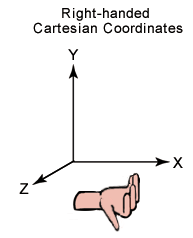
\includegraphics[width=\textwidth]{Bilder/Koordinatensystem.png}
\end{center}\end{column}
\end{columns}
\end{frame}

\subsection{FusionVis - Visualisierungstool}

\begin{frame}\frametitle{Darstellung von Daten im Visualisierungstool}
\begin{center}
	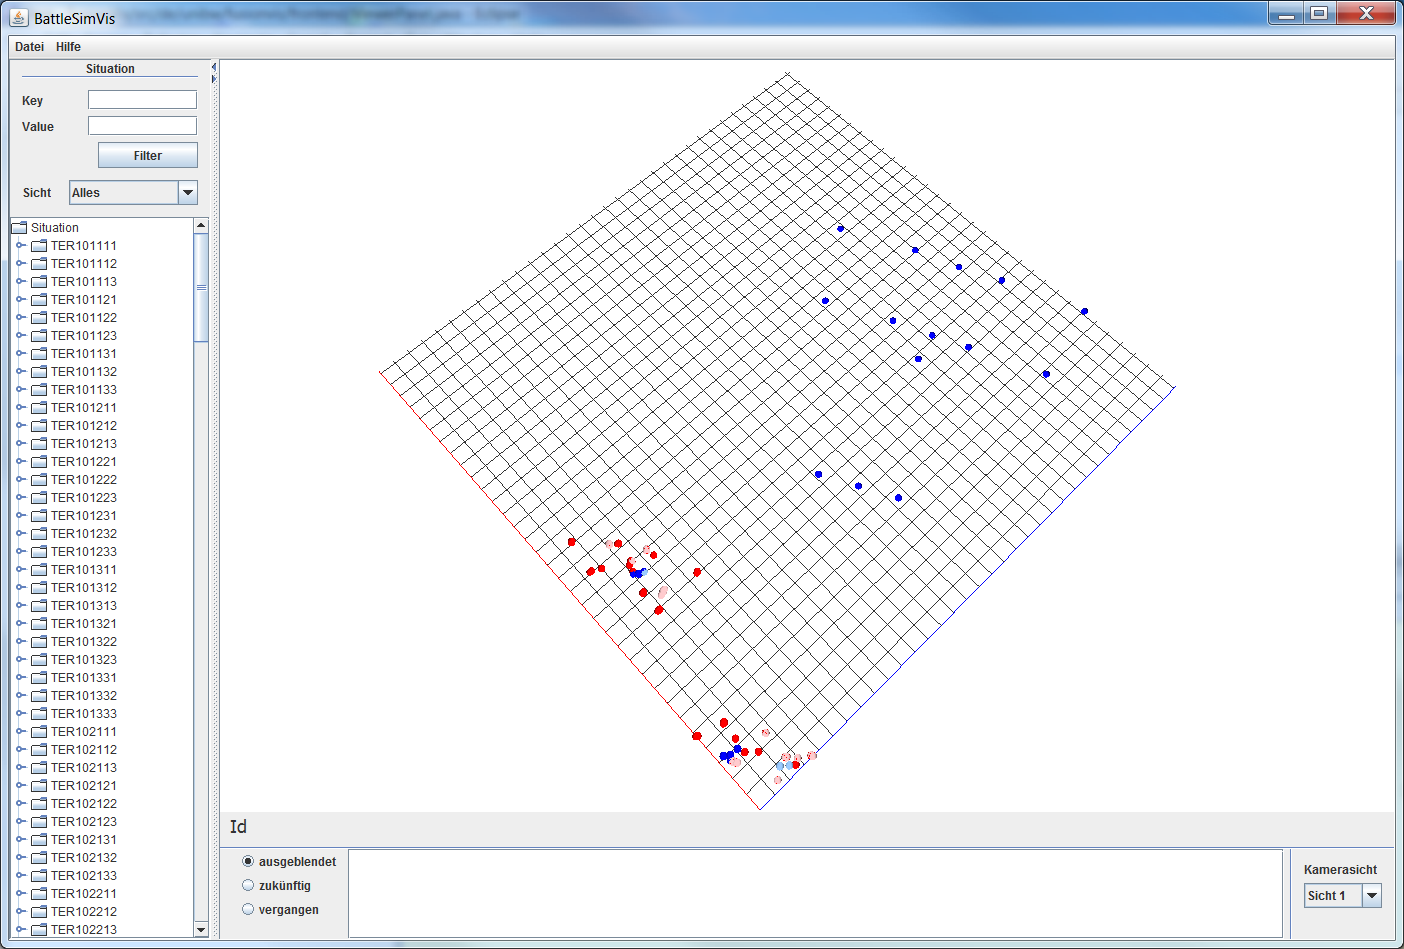
\includegraphics[width=0.7\textwidth]{Bilder/screen.png}
\end{center}
 %   \begin{itemize}
%        \item Freund-/Feind-Unterscheidung
%        \item Unterscheidung beobachtet/real
%        \item Kugel als Datenpunkt
%    \end{itemize}
\end{frame}


\begin{frame}\frametitle{Features}
 \begin{columns}[t]
\begin{column}{5cm}
    \begin{block}{}
    \begin{itemize}
        \item Plattformunabh�ngigkeit
        \item XML-Import
        \item strukturierte textuelle Datendarstellung (Baum)
        \item 3D-Darstellung der Daten
        \item voreingestellte Perspektiven
    \end{itemize}
    \end{block}
\end{column}
\begin{column}{5cm}
    \begin{block}{}
    \begin{itemize}
        \item freie Navigierbarkeit im 3D-Raum
        \item Klassifizierung durch Farben
        \item Datenfilter
        \item Selektion in der 3D-Darstellung
    \end{itemize}
    \end{block}
\end{column}
\end{columns}\end{frame}

\subsection{Fusion}
\begin{frame}\frametitle{Fusion durch Visualisierung}
  \begin{block}{Informationsfusion durch Visualisierung}
   \begin{enumerate}
   	\item ortsgleiche Sichtungen eines Objekts
   	
    \begin{itemize}
	    \item Daten am selben Ort befefinden sich an der selben Stelle
	    \item Ungenauigkeiten (Jitter) k�nnen als solche erkannt werden
     \end{itemize}
   	\item multiple Sichtungen eines Objekts zu unterschiedlichen Zeiten
   	\begin{itemize}
	    \item Annahme: Beobachtete Fahrzeuge haben eine Maximalgeschwindigkeit $v_{max}$
	    \item $v_{max}$ bestimmt die maximale Reichweite in gegebener Zeit
	    \item Reichweite eine Objektes vom Datenpunkt $p_{0}$ aus kann durch ein Volumen $K$ in Form eines Kegels dargestellt werden
	    \item F�r jeden Datenpunkt $p \neq p_{0}$ gilt:\\
	          $p\notin K \rightarrow p \quad ist \quad keine \quad Beobachtung \quad von \quad p_{0}$ 
    \end{itemize}
   \end{enumerate}
\end{block}\end{frame}

\begin{frame}\frametitle{Bewegungstrichter}
\end{frame}

